% Single-file submission generated by revision/manuscript/make_submission.py.
% Edit the sources in revision/manuscript/ instead.
\documentclass[pdflatex,sn-basic]{sn-jnl}
\usepackage{amsmath,amssymb,booktabs,graphicx,array}
\let\orcidlogo\relax% sn-jnl defines this via an absent Orcidlogo.eps
\usepackage{orcidlink}
\hypersetup{pdftitle={Nearest-neighbour distances and prediction error in spatial cross-validation},pdfauthor={Olatunji Johnson},pdfsubject={Research article}}
\newcommand{\E}{\mathbb{E}}
\newcommand{\Var}{\operatorname{Var}}
\newcommand{\Cov}{\operatorname{Cov}}
\newcommand{\CV}{\operatorname{CV}}
\newcommand{\R}{\mathbb{R}}
% Generated by revision/R/make_manuscript_numbers.R; do not edit.
\newcommand{\SignA}{87.09}
\newcommand{\SignSEA}{0.31}
\newcommand{\SignJOne}{97.86}
\newcommand{\SignSEJOne}{0.14}
\newcommand{\SignJTwo}{99.48}
\newcommand{\SignSEJTwo}{0.07}
\newcommand{\BiasA}{0.04171}
\newcommand{\BiasW}{0.04093}
\newcommand{\BiasJOne}{0.03660}
\newcommand{\BiasJTwo}{0.03566}
\newcommand{\BiasUOne}{0.03768}
\newcommand{\BiasUTwo}{0.03709}
\newcommand{\BiasRandom}{0.15903}
\newcommand{\BiasKnn}{0.04314}
\newcommand{\BiasOracle}{0.03527}
\newcommand{\BiasDelta}{-0.00527}
\newcommand{\BiasDeltaSE}{0.00017}
\newcommand{\BiasReduction}{12.9}
\newcommand{\BoundaryIsoLow}{23}
\newcommand{\BoundaryIsoHigh}{194}
\newcommand{\BoundaryAnisoLow}{76}
\newcommand{\BoundaryAnisoHigh}{153}
\newcommand{\SmallGapIso}{16.4}
\newcommand{\SmallCountIso}{444}
\newcommand{\SmallGapAniso}{14.2}
\newcommand{\SmallCountAniso}{742}
\newcommand{\SensAnisoEst}{90.6}
\newcommand{\SensAnisoNominal}{96.9}
\newcommand{\SensAnisoTrue}{99.9}
\newcommand{\CertAniso}{45.2}
\newcommand{\SizeAniso}{0.016}
\newcommand{\SensIsoEst}{93.0}
\newcommand{\SensIsoNominal}{99.3}
\newcommand{\SensIsoTrue}{99.3}
\newcommand{\CertIso}{29.8}
\newcommand{\SizeIso}{0.022}
\newcommand{\NeighbourCounterexample}{0.02306}
\newcommand{\ForestZero}{0.302}
\newcommand{\ForestZeroSE}{0.058}
\newcommand{\ForestNine}{0.013}
\newcommand{\ForestNineSE}{0.003}
\newcommand{\IDWZero}{0.500}
\newcommand{\IDWZeroSE}{0.028}
\newcommand{\IDWNine}{0.486}
\newcommand{\IDWNineSE}{0.022}
\newcommand{\KrigingZero}{0.427}
\newcommand{\KrigingZeroSE}{0.020}
\newcommand{\KrigingNine}{0.001}
\newcommand{\KrigingNineSE}{0.001}
\newcommand{\LinearZero}{0.265}
\newcommand{\LinearZeroSE}{0.053}
\newcommand{\LinearNine}{0.001}
\newcommand{\LinearNineSE}{0.001}
\newcommand{\ConstantMarginal}{0.388}
\newcommand{\JuraPublishedRandomScore}{0.279}
\newcommand{\JuraPublishedRandomJTwo}{0.159}
\newcommand{\JuraPublishedRandomW}{0.1191}
\newcommand{\JuraPublishedRandomMAE}{0.042}
\newcommand{\JuraPublishedTarget}{0.322}
\newcommand{\JuraPublishedBlockScore}{0.545}
\newcommand{\JuraPublishedBlockJTwo}{-0.132}
\newcommand{\JuraPublishedBlockW}{0.5107}
\newcommand{\JuraPublishedBlockMAE}{0.224}
\newcommand{\JuraPublishedBufferScore}{0.545}
\newcommand{\JuraPublishedBufferJTwo}{-0.132}
\newcommand{\JuraPublishedBufferW}{0.5107}
\newcommand{\JuraPublishedBufferMAE}{0.224}
\newcommand{\JuraPublishedKnnScore}{0.443}
\newcommand{\JuraPublishedKnnJTwo}{-0.030}
\newcommand{\JuraPublishedKnnW}{0.0377}
\newcommand{\JuraPublishedKnnMAE}{0.122}
\newcommand{\JuraUniformRandomScore}{0.310}
\newcommand{\JuraUniformRandomJTwo}{-0.004}
\newcommand{\JuraUniformRandomW}{0.0158}
\newcommand{\JuraUniformRandomMAE}{0.054}
\newcommand{\JuraUniformTarget}{0.288}
\newcommand{\JuraUniformBlockScore}{0.491}
\newcommand{\JuraUniformBlockJTwo}{-0.166}
\newcommand{\JuraUniformBlockW}{0.5499}
\newcommand{\JuraUniformBlockMAE}{0.203}
\newcommand{\JuraUniformBufferScore}{0.492}
\newcommand{\JuraUniformBufferJTwo}{-0.167}
\newcommand{\JuraUniformBufferW}{0.5517}
\newcommand{\JuraUniformBufferMAE}{0.204}
\newcommand{\JuraUniformKnnScore}{0.312}
\newcommand{\JuraUniformKnnJTwo}{-0.004}
\newcommand{\JuraUniformKnnW}{0.0149}
\newcommand{\JuraUniformKnnMAE}{0.054}
\newcommand{\JuraNorthRandomScore}{0.289}
\newcommand{\JuraNorthRandomJTwo}{0.167}
\newcommand{\JuraNorthRandomW}{0.7352}
\newcommand{\JuraNorthRandomMAE}{0.237}
\newcommand{\JuraNorthTarget}{0.526}
\newcommand{\JuraNorthBlockScore}{0.396}
\newcommand{\JuraNorthBlockJTwo}{0.003}
\newcommand{\JuraNorthBlockW}{0.2706}
\newcommand{\JuraNorthBlockMAE}{0.130}
\newcommand{\JuraNorthBufferScore}{0.396}
\newcommand{\JuraNorthBufferJTwo}{0.003}
\newcommand{\JuraNorthBufferW}{0.2706}
\newcommand{\JuraNorthBufferMAE}{0.130}
\newcommand{\JuraNorthKnnScore}{0.358}
\newcommand{\JuraNorthKnnJTwo}{0.013}
\newcommand{\JuraNorthKnnW}{0.3888}
\newcommand{\JuraNorthKnnMAE}{0.169}
\newcommand{\NestedMAEW}{0.15251}
\newcommand{\NestedBiasW}{-0.03461}
\newcommand{\NestedMAEJTwo}{0.14902}
\newcommand{\NestedBiasJTwo}{-0.01479}
\newcommand{\NestedMAEKnn}{0.15334}
\newcommand{\NestedBiasKnn}{-0.03176}
\newcommand{\NestedMAERandom}{0.22569}
\newcommand{\NestedBiasRandom}{0.19030}
\newcommand{\NestedDelta}{-0.00349}
\newcommand{\NestedSE}{0.00152}
\newcommand{\NestedLower}{-0.00647}
\newcommand{\NestedUpper}{-0.00051}
\newcommand{\NestedReduction}{2.3}
\newcommand{\NestedShiftDelta}{-0.01436}
\newcommand{\NestedShiftSE}{0.00500}
\newcommand{\NestedStrongCellDelta}{-0.07951}
\newcommand{\NestedOtherCellsDelta}{-0.00018}
\newcommand{\NestedSameChoices}{1141}
\newcommand{\NestedWins}{394}
\newcommand{\NestedLosses}{385}
\newcommand{\NestedOmissionMin}{-0.00390}
\newcommand{\NestedOmissionMax}{-0.00294}
\newcommand{\NestedStrongRandomChoices}{53}
\newcommand{\NestedStrongWRandomChoices}{0}
\newcommand{\NestedStrongTargetRisk}{0.862}
\newcommand{\NestedStrongCVRandom}{0.790}
\newcommand{\NestedStrongCVKnn}{1.034}
\raggedbottom
\begin{document}
\title[Nearest-neighbour distances and prediction error]{Nearest-neighbour distances and prediction error in spatial cross-validation}
\author*[1]{\fnm{Olatunji} \sur{Johnson}\,\orcidlink{0000-0002-4080-0999}}\email{olatunji.johnson@manchester.ac.uk}
\affil*[1]{\orgdiv{Department of Mathematics}, \orgname{University of Manchester}, \orgaddress{\street{Oxford Road}, \city{Manchester}, \postcode{M13 9PL}, \country{United Kingdom}}}
\abstract{Cross-validation (CV) can underestimate spatial prediction error when validation observations are closer to training data than the intended prediction locations. We ask whether spatial correlation improves the choice of CV scheme beyond distance matching. We define $J_2$ as the difference between validation and target locations in their average squared correlation with the nearest training observation. For Gaussian prediction using one neighbour, with known mean and covariance, multiplying $J_2$ by response variance gives target mean squared error (MSE) minus expected CV MSE. Additional training observations can reduce prediction error further, by different amounts at validation and target locations. We derive this difference, which can produce CV bias even when nearest-distance distributions match exactly. Among four CV schemes, selection by $|J_2|$ reduced mean absolute expected bias by \BiasReduction\% relative to selection by the Wasserstein distance across 5,120 configurations with known covariance. In 1,920 datasets with estimated covariance, the reduction in mean absolute error of the observed CV estimate was \NestedReduction\%. Almost all of this gain came from one setting: uniform sampling, rapidly decaying correlation, low noise and a target extending beyond the sampled region. A ten-fold check gave a 1.7\% reduction, with a Monte Carlo interval that included zero. Predictors can also change CV bias while response covariance remains fixed. In a soil-cadmium application, both diagnostics select k-fold nearest-neighbour distance matching, but random CV is closer to the observed prediction error at 100 reserved sites. Nearest-neighbour correlation alone cannot determine CV bias when prediction uses several neighbours or predictors.}
\keywords{Gaussian process, kriging, map accuracy, screening effect, spatial autocorrelation, Wasserstein distance}
\maketitle
\section{Introduction}
Spatial prediction models are often used to estimate responses at locations where observations are unavailable. Assessing their prediction error requires a validation procedure that represents the intended prediction task. Cross-validation (CV) estimates error by holding out groups of observations, fitting the prediction model to the remaining data, and comparing predictions with the held-out responses. However, the spatial relationships created by these splits can differ from those encountered when the final prediction model is applied. With clustered sampling, validation observations may have close training neighbours while much of the prediction area lies farther from the data. Conversely, holding out large spatial blocks can create greater separations than the final prediction task requires. These differences can affect how well CV estimates target prediction error.

Nearest-neighbour distance matching uses the prediction locations to guide the choice of validation training sets. \citet{mila2022nndm} proposed NNDM leave-one-out CV, which selectively excludes nearby training observations to match validation and target nearest-distance distributions over distances within an autocorrelation range. \citet{linnenbrink2024knndm} extended this approach to $k$-fold CV through kNNDM. It compares candidate fold configurations using the Wasserstein distance $W$, an established measure of the difference between probability distributions \citep{panaretos2019wasserstein}. Here, $W$ measures the total area between the cumulative distributions of validation and target nearest-training distances. Choosing a smaller $W$ brings these two distributions closer together.

The usefulness of nearby training observations also depends on the prediction model and its predictors. Spatial prediction error profiles estimate how a particular model's observed error changes with distance from training data \citep{brenning2023profiles}. They can reveal whether increasing separation is associated with increasing error for that model. Geographic proximity alone also cannot establish whether predictor values at a target location are represented in training. Area-of-applicability methods assess this aspect of prediction by comparing target predictor values with those in the training data \citep{meyer2021aoa}.

Other spatial validation methods adjust CV scores to account for correlation or differences between the sampled and target locations. Covariance-based corrections account for correlated responses \citep{rabinowicz2022correlated,yuval2025classification}. Sampling-intensity weights, spatial modelling of validation residuals, and importance weights combined with exclusion buffers address differences between the sampled sites and the prediction target \citep{debruin2022clustered,wang2023geospatial}. Dissimilarity-adaptive CV combines random and spatial CV scores according to predictor similarity \citep{wang2025dissimilarity}, while target-weighted CV weights validation losses to represent target characteristics \citep{brenning2026targetweighted}.

For distance matching, the central question is how a difference in nearest-training distance translates into a difference in prediction error. The Wasserstein distance describes the geographic difference without using the strength of correlation at each separation. For a prediction model that uses spatial dependence, increasing separation matters when it removes useful information from neighbouring responses. If responses are already weakly correlated at both distances, a larger separation may have little effect. Where correlation decreases rapidly, a smaller change in distance may remove more information. This suggests evaluating distance matching through its relationship with spatial correlation and the prediction model's mean squared error (MSE).

Our first contribution is an explicit connection between nearest-neighbour correlation and MSE. For Gaussian prediction using one neighbour, with known mean and covariance, the reduction in MSE is proportional to the squared correlation with that observation. This motivates $J_2$, which subtracts the average squared correlation at target locations from the corresponding average during validation. Using standard Gaussian conditioning \citep{rasmussen2006gpml}, we show that response variance multiplied by $J_2$ is exactly target MSE minus expected CV MSE.

Our second contribution is to quantify what a nearest-neighbour comparison leaves out. When Gaussian prediction uses all training observations, the remaining neighbours can reduce error beyond what the nearest observation alone achieves. We derive how this additional reduction differs between validation and target locations. This difference can have either sign and forms the part of expected CV bias that $J_2$ does not capture. A leave-one-out counterexample gives identical nearest-distance distributions but nonzero expected CV bias. The result explains why even perfect nearest-distance matching may be insufficient when prediction uses several observations.

Our third contribution is to test whether selecting CV schemes using correlation gives more accurate estimates of target prediction error. We compare selection by the smallest $|J_2|$ with selection by the smallest $W$ among random folds, spatial blocks, buffered spatial blocks and kNNDM. Studies with known and estimated covariance assess expected bias and the accuracy of the observed CV error estimate. Further simulations vary the prediction model and the information supplied by predictors while holding response covariance fixed. An application predicts continuous soil-cadmium concentrations in the Swiss Jura and compares the selected CV estimates with measured prediction error at reserved sites.

Section~\ref{sec:methods} defines the prediction target and diagnostics, derives their relationships with MSE, and describes the CV selection rules. Section~\ref{sec:simulation} presents the simulation designs and results. Section~\ref{sec:application} presents the Swiss Jura application and its findings. Section~\ref{sec:discussion} discusses the implications for choosing and interpreting spatial CV schemes.
\section{Methods}
\label{sec:methods}
\subsection{Prediction target and error measures}
Let $S=\{s_1,\ldots,s_n\}$ denote the locations of the observed training responses. Write $\widehat m_T(t)$ for the prediction at location $t$ from a prediction model fitted using observations at $T$. The final prediction model uses all observations at $S$; CV fits the same type of prediction model to subsets of these observations.

The target distribution $Q$ specifies where prediction error is evaluated and how errors at those locations are averaged. For a target grid $\{t_1,\ldots,t_M\}$, assign nonnegative weights $q_1,\ldots,q_M$ that sum to one. The squared error at $t_j$ is multiplied by $q_j$ before the errors are added. With equal weights, $q_j=1/M$, so target error is the ordinary average of the errors at the $M$ grid points. This defines error at those points. Using that average to approximate error across an entire region requires a grid and weights that represent the whole region.

For one CV partition, the disjoint test folds $H_1,\ldots,H_K$ together contain all locations in $S$. Fold $f$ trains on a nonempty set $T_f\subseteq S\setminus H_f$ and predicts the responses at $H_f$. Ordinary CV uses $T_f=S\setminus H_f$ \citep{arlot2010survey}. With buffering, observations within a specified distance of any test location are also removed from that fold's training set. This changes the training set while leaving its test fold unchanged. Each observation therefore supplies one held-out prediction, and the observed CV MSE (the CV score) $\widehat C$ is the average of the resulting $n$ squared errors:
\[
 \widehat C=\frac{1}{n}\sum_f\sum_{i\in H_f}[Y(s_i)-\widehat m_{T_f}(s_i)]^2.
\]
Thus each test observation contributes with weight $1/n$, even when the folds have different sizes.

MSE, or \emph{risk}, is the expected squared difference between a response and its prediction. Here, $\E_Y$ averages over possible datasets of training and target responses from the same spatial model, including observation noise. Prediction models are refitted for each dataset. Locations, target weights and CV folds are chosen without using response values and held fixed.

At a target location, $Y(t)$ denotes the response to be predicted, including observation noise. If a target location coincides with a training location, it represents a new measurement with independent observation noise. Define the target MSE $R_Q$, expected CV MSE $C$, and their difference $O$ as
\begin{align}
 R_Q &= \E_Y\E_{t\sim Q}\{[Y(t)-\widehat m_S(t)]^2\},\\
 C &= \E_Y(\widehat C),\qquad O=R_Q-C.\label{eq:risk}
\end{align}
Here $\E_{t\sim Q}$ averages over target locations; on a finite grid, it weights the error at $t_j$ by $q_j$. A positive $O$ means that CV underestimates target MSE on average, and a negative $O$ means that it overestimates it. We call $O$ \emph{optimism}; the usual estimator bias is $C-R_Q=-O$. The difference reflects both the locations used for validation and the smaller training sets used within CV.

For a particular observed dataset, the relevant target MSE keeps its training responses $Y_S$ and fitted prediction model fixed, and averages over possible target responses conditional on $Y_S$ \citep{bates2024crossvalidation}. Denote this conditional target MSE by
\[
 R_Q(Y_S)=\E_{t\sim Q}\E\bigl\{[Y(t)-\widehat m_S(t)]^2\mid Y_S\bigr\}.
\]
The difference $R_Q(Y_S)-\widehat C$ measures the error of that dataset's CV estimate. A small $|O|$ can coexist with large errors for individual datasets, because underestimation in some datasets can cancel overestimation in others.

The known-covariance experiment calculates $O$ analytically and compares selection rules using the average of $|O|$ across location configurations. The experiment with estimated covariance instead calculates $|R_Q(Y_S)-\widehat C|$ for each simulated dataset and averages these absolute errors. It therefore assesses how accurately the observed CV MSE estimates the conditional target MSE of the prediction model fitted to that dataset.

\subsection{Nearest-neighbour distance distributions}
\label{sec:distances}
Following nearest-neighbour distance matching \citep{mila2022nndm,linnenbrink2024knndm}, we compare validation and target nearest-training distances. For each validation observation at $s_i\in H_f$, define its nearest-training distance as
\[
 d_i^C=\min_{s\in T_f}\|s_i-s\|,
\]
where $\|s_i-s\|$ is the Euclidean distance between the two locations. The distance is measured from the validation location $s_i$ to the nearest observation available in its fold's training set $T_f$. The search excludes all observations in the test fold and any observations removed by the buffer. This gives one distance $d_i^C$ for each of the $n$ validation observations.

Let $D_C$ denote the distance obtained by choosing one validation observation uniformly from these $n$ observations. Thus $d_i^C$ is the distance for a particular observation, while $D_C$ describes the variation in these distances across validation observations, each with weight $1/n$. The calculation starts from each validation location; starting from each training location and finding its nearest validation observation would define a different distribution.

For each target grid point $t_j$, define
\[
 d_j^Q=\min_{s\in S}\|t_j-s\|.
\]
This is the distance from $t_j$ to its nearest observation in the full training set $S$. Let $D_Q$ denote this distance for a target location drawn from $Q$. On a finite target grid, location $t_j$ contributes its distance $d_j^Q$ with weight $q_j$. With equal target weights, each of the $M$ locations has weight $1/M$.

Let $F_C(u)=\Pr(D_C\leq u)$ and $F_Q(u)=\Pr(D_Q\leq u)$ be the cumulative distribution functions (CDFs). Here $F_C(u)$ is the proportion of validation observations whose nearest available training observation is at most distance $u$ away. On a finite target grid, $F_Q(u)$ is the sum of the weights $q_j$ for target locations whose nearest observation in $S$ is at most distance $u$ away. With equal weights, this is the proportion of target locations satisfying that condition. Figure~\ref{fig:diagnostic}A shows an example set of observation and target locations; Figure~\ref{fig:diagnostic}B compares their distance CDFs under random and blocked CV.

For finite mean distances, two useful summaries are
\begin{equation}
 A=\E D_Q-\E D_C=\int_0^\infty(F_C-F_Q)\,du,\qquad
 W=\int_0^\infty|F_C-F_Q|\,du.\label{eq:geometry}
\end{equation}
The expectations here average distances over validation observations or target locations, using their respective weights. The mean-distance difference $A$ is positive when target locations are farther from training observations on average. The Wasserstein distance $W$ measures the total area between the two CDFs \citep{panaretos2019wasserstein}. It is zero only when the distance distributions match. Both quantities have distance units.

The distinction between $A$ and $W$ becomes important when the CDFs cross. Positive and negative values of $F_C-F_Q$ can cancel in $A$, whereas their absolute values add to $W$. Consequently, equal mean distances can conceal different distributions. In general, $|A|\leq W$; equality holds when the CDF difference has the same sign almost everywhere.

\subsection{Correlation model and contrasts}
\label{sec:correlation-model}
The distance distributions describe how close validation and target locations are to training observations. To describe the strength of dependence at these distances, we use a Gaussian spatial model with independent observation noise \citep[Chapter~2]{rasmussen2006gpml}. Consider
\[
 Y(s)=\mu(s)+Z(s)+\epsilon(s),
\]
where $\mu(s)$ is a known mean and $Z(s)$ is a mean-zero, stationary, isotropic Gaussian spatial process with variance $\sigma^2$ and correlation function $r(u)$. Its covariance depends only on the separation distance $u$. The observation noise $\epsilon(s)$ is mean-zero Gaussian with variance $\tau^2$, independent between measurements and independent of $Z$. Each response therefore has total variance $V=\sigma^2+\tau^2>0$.

For two distinct measurements separated by distance $u$, the covariance is $\sigma^2r(u)$ because the independent noise contributes no covariance. Their correlation is consequently
\[
 \rho(u)=\frac{\sigma^2r(u)}{\sigma^2+\tau^2}=wr(u),
 \qquad w=\frac{\sigma^2}{V}.
\]
Here $r(u)$ is the correlation within the spatial process, whereas $\rho(u)$ is the correlation between the observed responses, including noise. The fraction $w$ is the proportion of response variance attributable to the spatial process. These parameters may be specified in a simulation or estimated from training responses.

For exponential spatial correlation, $r(u)=\exp(-u/\phi)$ and $\rho(u)=w\exp(-u/\phi)$, where $\phi>0$ is a distance scale. At $u=\phi$, the correlation within the spatial process is $r(\phi)=\exp(-1)\approx0.368$. The correlation between observed responses is $\rho(\phi)=w\exp(-1)\approx0.368w$. Larger values of $\phi$ give slower decay; the exponential spatial correlation remains positive at every finite distance. For distinct measurements at the same location, $\rho(0)=w$ because their observation noise is independent. A measurement's correlation with itself is one; the target response here is a separate measurement even when its location coincides with a training location.

We apply the same function $\rho$ to the validation and target distances. The quantities $\rho(D_C)$ and $\rho(D_Q)$ are the correlations implied by this model between a response and its nearest available training response during validation and target prediction, respectively. Their expectations average over the distance distributions defined above, with the correlation function held fixed.

Using the individual distances defined in Section~\ref{sec:distances}, $\rho(d_i^C)$ is the correlation between validation response $Y(s_i)$ and its nearest training response in $T_f$. Similarly, $\rho(d_j^Q)$ is the correlation between the target response at $t_j$ and its nearest training response in $S$. Their averages are
\[
\begin{aligned}
 \E\{\rho(D_C)\}&=\frac{1}{n}\sum_{i=1}^n \rho(d_i^C),
 &\E\{\rho(D_Q)\}&=\sum_{j=1}^M q_j \rho(d_j^Q),\\[4pt]
 \E\{[\rho(D_C)]^2\}&=\frac{1}{n}\sum_{i=1}^n [\rho(d_i^C)]^2,
 &\E\{[\rho(D_Q)]^2\}&=\sum_{j=1}^M q_j[\rho(d_j^Q)]^2.
\end{aligned}
\]
The first row gives the average correlation during validation and at the target. The second row squares each correlation before averaging. Validation observations have equal weights $1/n$; target locations use the weights $q_j$ specified by $Q$. For equally weighted target locations, $q_j=1/M$.

We define the \emph{correlation contrasts} as the differences between the corresponding validation and target averages:
\begin{equation}
 J_1=\E\{\rho(D_C)\}-\E\{\rho(D_Q)\},\qquad
 J_2=\E\{[\rho(D_C)]^2\}-\E\{[\rho(D_Q)]^2\}.\label{eq:indices}
\end{equation}
Both contrasts are dimensionless. A positive $J_2$ means that the average squared correlation with the nearest available training response is higher for validation observations than for target locations. A negative $J_2$ means that this average is higher for target locations than for validation observations. A value of zero means that the two averages are equal. The same sign interpretation applies to $J_1$ using correlations rather than squared correlations. The squared form is motivated by the connection to MSE derived in Section~\ref{sec:one-neighbour} for Gaussian prediction using one neighbour with known mean and covariance.

\subsection{Correlation weighting and distance matching}
The correlation contrasts can also be written in terms of the distance CDFs. This shows how they differ from the Wasserstein distance $W$. For the exponential response correlation $\rho(u)=w\exp(-u/\phi)$, integration by parts gives
\begin{equation}
\begin{aligned}
 J_2&=\int_0^\infty\lambda_2(u)\{F_C(u)-F_Q(u)\}\,du,\\
 \lambda_2(u)&=-\frac{d}{du}[\rho(u)^2]
 =\frac{2w^2}{\phi}\exp(-2u/\phi).
\end{aligned}
\label{eq:weighting}
\end{equation}
The weight $\lambda_2(u)$ measures how rapidly squared correlation decreases with distance. For the exponential model with $w>0$, it is largest at short distances and decreases as $u$ increases. Differences between the two CDFs therefore receive more weight at short distances. This is what we mean by \emph{correlation weighting}. Figure~\ref{fig:diagnostic}C shows the weights for $J_1$ and $J_2$.

A CV scheme specifies the test folds and their training sets. We compare schemes by choosing the smallest $W$ or $|J_2|$. The distance $W$ adds absolute CDF differences equally per unit distance; $J_2$ adds signed differences weighted by $\lambda_2(u)$. When the CDFs cross, positive and negative contributions can offset one another: \emph{cancellation}. Taking the absolute value after integration preserves this cancellation. The two criteria therefore differ in both weighting and cancellation; a small $|J_2|$ need not mean similar distance distributions.

To examine weighting without cancellation, we also evaluate
\[
 U_2=\int_0^\infty\lambda_2(u)|F_C(u)-F_Q(u)|\,du.
\]
This measure uses the same weights as $J_2$ but takes absolute differences before adding them. It is the Wasserstein distance between the distributions of squared correlations, $[\rho(D_C)]^2$ and $[\rho(D_Q)]^2$. The corresponding measure $U_1$ compares the distributions of unsquared correlations. Both measures are nonnegative and satisfy $|J_p|\leq U_p$ for $p=1,2$; Online Resource 1 (Section~S3.1) gives their general integral expressions.

Weak spatial signal can make the contrasts small even when validation and target distance distributions differ substantially. For a fixed spatial correlation function $r$ shared by all CV schemes, their common signal fraction $w>0$ scales every $J_p$ by $w^p$. Reducing $w$ therefore shrinks the contrasts without changing which scheme has the smallest $|J_p|$.

\begin{figure}[p]
\centering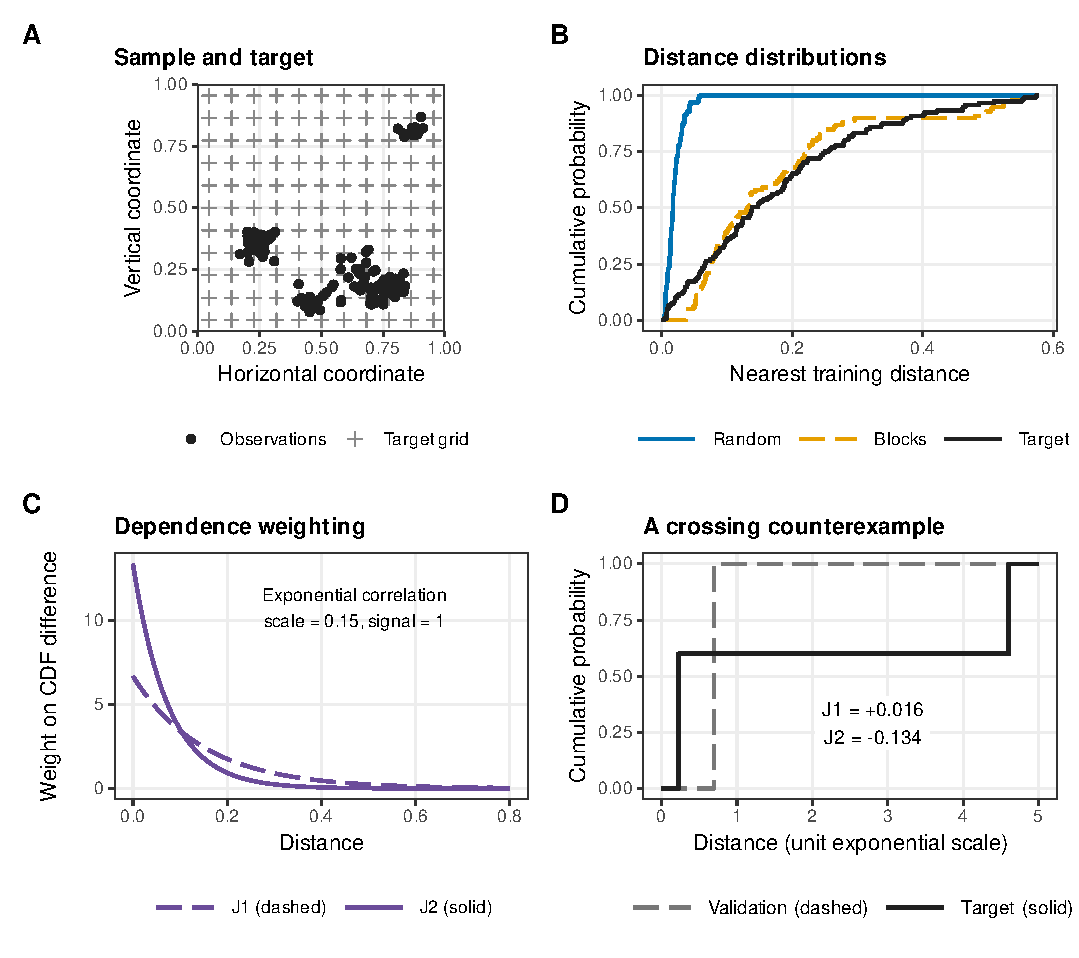
\includegraphics[width=\textwidth]{Fig1.pdf}
\caption{From nearest-training distances to correlation contrasts. (A) Example observation locations (black circles) and target grid (grey crosses). (B) Distance CDFs for random CV (blue solid), blocked CV (orange dashed) and target prediction (black solid). (C) Weights applied to the CDF difference for $J_1$ (dashed) and $J_2$ (solid), using exponential scale $0.15$ and signal fraction one. (D) A separate example in which the validation CDF (grey dashed) and target CDF (black solid) cross, giving $J_1$ and $J_2$ opposite signs. Panels C and D illustrate specified correlation functions; they do not estimate covariance from panel A. Panel D uses unit exponential scale.}
\label{fig:diagnostic}
\end{figure}

\clearpage
\subsection{Exact MSE difference for prediction using one neighbour}
\label{sec:one-neighbour}
The squared contrast $J_2$ gives an exact MSE difference when prediction uses only the nearest training response. Assume the Gaussian model in Section~\ref{sec:correlation-model}, with known mean and covariance and the same observation-noise variance at training and target locations. If the nearest training response is at $s_*$, a distance $D$ from $t$, Gaussian conditioning gives the prediction that minimises MSE \citep[Chapter~2]{rasmussen2006gpml}:
\[
 \widehat m_T(t)=\mu(t)+\rho(D)\{Y(s_*)-\mu(s_*)\}.
\]
The neighbour's departure from its mean adjusts the mean at $t$, in proportion to their response correlation. The MSE is $V\{1-\rho(D)^2\}$: squared correlation determines how much the neighbour reduces prediction error.

Averaging over target distances gives $V[1-\E\{\rho(D_Q)^2\}]$; averaging over validation distances gives $V[1-\E\{\rho(D_C)^2\}]$. Subtracting expected CV MSE from target MSE therefore gives
\begin{equation}
 O_1=VJ_2.\label{eq:one}
\end{equation}
Here $O_1$ is the optimism defined in equation~\eqref{eq:risk} for this one-neighbour prediction model. Positive $J_2$ means that CV underestimates target MSE; negative $J_2$ means that it overestimates it. Under these assumptions, choosing the CV scheme with the smallest $|J_2|$ also minimises $|O_1|$. These MSEs average over possible training and target responses while keeping locations, folds and target weights fixed. Adding $VJ_2$ removes the average bias of CV under this one-neighbour model. For an individual dataset, the adjusted score can still overestimate or underestimate the fitted model's conditional target MSE.

The distance CDFs can also establish the sign. Suppose response correlation is nonnegative and does not increase with distance. If $F_C(u)\geq F_Q(u)$ for every $u$, validation observations are at least as likely as target locations to have a training neighbour within any specified distance. Then $J_1,J_2,O_1\geq0$: CV underestimates target MSE or equals it. Reversing the CDF ordering reverses the inequalities. Different distance distributions can still give equality where correlation is constant, including when there is no spatial signal.

When the CDFs cross, $J_1$ and $J_2$ can have opposite signs (Figure~\ref{fig:diagnostic}D). Let $m_C,m_Q$ be the means of the validation and target correlations, and $v_C,v_Q$ their variances. Then
\begin{equation}
 J_2=(m_C+m_Q)J_1+v_C-v_Q.\label{eq:moments}
\end{equation}
Thus $J_1$ compares average correlations but omits their difference in variance. For example, suppose validation correlation is always $0.5$, while target correlation is $0.8$ with probability $0.6$ and $0.01$ otherwise. These values are possible under an exponential model and give $J_1=0.016$ but $J_2=-0.13404$. Despite positive $J_1$, CV overestimates target MSE in this example because $O_1=VJ_2<0$.



\subsection{Prediction using all available training observations}
The remaining training observations can supply information beyond the nearest neighbour. Under the same Gaussian model with known mean and covariance, the optimal prediction using all available training observations is simple kriging. Let $Y_T$ be the vector of responses at training locations $T$, $\Sigma_T=\Cov(Y_T)$ their covariance matrix, and $b(t,T)=\Cov(Y_T,Y(t))$ the vector of their covariances with the response to be predicted. If $\Sigma_T$ is nonsingular, the MSE is $V-e(t,T)$, where
\[
 e(t,T)=b(t,T)^\top\Sigma_T^{-1}b(t,T).
\]
Thus $e(t,T)$ is the reduction in MSE supplied jointly by the training observations \citep{rasmussen2006gpml}. Positive observation-noise variance is sufficient for $\Sigma_T$ to be nonsingular.

Let $D(t,T)$ be the nearest distance from $t$ to $T$. Using only that nearest observation reduces MSE by $V\rho[D(t,T)]^2$. The additional reduction supplied by the remaining observations is therefore
\[
 a(t,T)=e(t,T)-V\rho[D(t,T)]^2\geq0.
\]
This quantity is nonnegative because the optimal prediction using all observations could always assign zero weight to the others and reproduce the one-neighbour prediction.

For validation, denote the average total MSE reduction by $\overline{e}_C$ and the average additional reduction beyond the nearest neighbour by $\overline{a}_C$. Each observation has weight $1/n$ and is evaluated using its fold's training set. The corresponding target averages, $\E_Q e(t,S)$ and $\E_Q a(t,S)$, use the target weights in $Q$ and all training observations at $S$.

Expected CV MSE is $V-\overline{e}_C$, and target MSE is $V-\E_Q e(t,S)$. Subtracting expected CV MSE from target MSE cancels the common variance $V$, giving
\begin{equation}
\begin{aligned}
 O_{\mathrm{full}}&=\overline e_C-\E_Q e(t,S)\\
 &=VJ_2+\overline a_C-\E_Q a(t,S).
\end{aligned}
\label{eq:remainder}
\end{equation}
The first term, $VJ_2$, is the MSE difference for prediction using only the nearest neighbour. The remainder, $\overline{a}_C-\E_Q a(t,S)$, measures how much more the other observations reduce MSE during validation than at the target. A positive remainder increases optimism; a negative remainder decreases it. Thus $VJ_2$ alone gives the full MSE difference only when these additional benefits are equal on average.

Matching nearest distances can still leave CV biased. Place observations at $-1$, $0$ and $1$ on a line, and predict at $2$. Leave-one-out CV predicts each observation from the other two; target prediction uses all three. All nearest-training distances are one, so $W=J_1=J_2=0$. When predicting the held-out observation at $0$, both training observations are one unit away. At the target location $2$, only one training observation is one unit away; the others are two and three units away. With $V=1$, $w=0.8$ and $r(u)=\exp(-u)$, these additional neighbours reduce MSE more during validation, on average, than at the target. Thus $O_{\mathrm{full}}=\NeighbourCounterexample>0$: expected CV MSE is lower than target MSE. The difference comes entirely from the additional-neighbour term in equation~\eqref{eq:remainder}; Online Resource 1 (Section~S2.3) gives the calculation.

\subsection{Bounding the contribution of the other neighbours}
A bound on the additional MSE reduction $a(t,T)$ limits how far the full MSE difference can depart from $VJ_2$. We retain the Gaussian model with known mean and covariance.

Let $Y_1$ be the nearest training response and $Y_R$ the vector of remaining training responses. Write $b_1=\Cov(Y_1,Y(t))$, $b_R=\Cov(Y_R,Y(t))$ and $\Sigma_{R1}=\Cov(Y_R,Y_1)$. Then $\widetilde b_R=b_R-\Sigma_{R1}b_1/V$ contains the covariances between $Y_R$ and $Y(t)$ after conditioning on $Y_1$ \citep[Appendix~A.2]{rasmussen2006gpml}: the dependence remaining once the nearest response is known. For positive observation-noise variance, $\tau^2>0$,
\begin{equation}
 0\leq a(t,T)\leq B(t,T)
 =\min\{\|\widetilde b_R\|^2/\tau^2,\ \sigma^2-b_1^2/V\}.\label{eq:extra-bound}
\end{equation}
Here $\|\widetilde b_R\|^2$ is the sum of the squared entries of $\widetilde b_R$. The first upper bound follows because the remaining observations retain independent noise with variance $\tau^2$. The second is the spatial variance left after the nearest observation has reduced MSE by $b_1^2/V$; independent target noise cannot be predicted. Both limits apply, so $B$ takes the smaller one. Online Resource 1 (Sections~S3.2.1--S3.2.3) gives the pointwise proof.

Let $\overline{B}_C$ be the validation average of $B$, with each observation weighted by $1/n$ and evaluated using its fold's training set. The target average uses $Q$ and the full set $S$. In equation~\eqref{eq:remainder}, the additional validation reduction is added to $VJ_2$, while the additional target reduction is subtracted. Averaging these bounds (Online Resource 1, Section~S3.2.4) gives
\begin{equation}
 VJ_2-\E_Q B(t,S)\leq O_{\mathrm{full}}
 \leq VJ_2+\overline B_C.\label{eq:certificate}
\end{equation}
A positive lower limit guarantees that CV underestimates target MSE on average; a negative upper limit guarantees overestimation. If the interval includes zero, it does not establish a nonzero bias. These are deterministic limits under the known covariance model, rather than a confidence interval. Computing $B$ requires covariances involving all training observations, beyond the nearest distances alone.

For other prediction models, ordered distance distributions imply an MSE ordering only under additional conditions. One sufficient condition is that MSE does not decrease as nearest distance increases, following the same function during validation and target prediction (Online Resource 1, Section~S4). Sections~\ref{sec:sim-covariance} and~\ref{sec:sim-learners} examine the effects of covariance estimation, training size and prediction model; Section~\ref{sec:sim-refitting} tests selection by $|J_2|$ when covariance is estimated.

\subsection{CV schemes and selection rules}
\label{sec:cv-selection}
Each CV scheme defines test folds and their training sets. We compare four candidates, each with five folds. Balanced random folds assign observations randomly to groups of nearly equal size \citep{arlot2010survey}. Spatial blocks use coordinate $k$-means \citep{hartigan1979kmeans} to form geographic groups. Buffered spatial blocks retain the same test folds but remove training observations within the specified buffer distance of any test observation \citep{roberts2017cross}. kNNDM, implemented in CAST 1.1.1, constructs folds to bring validation and target nearest-training distance distributions closer together \citep{linnenbrink2024knndm}. These fold constructions use locations alone. The final prediction model is fitted to all available training observations.

A selection rule chooses among these four candidates using one diagnostic. For each simulation dataset or location configuration, we calculate the diagnostic for every candidate. Selection by $A$, $J_1$ or $J_2$ chooses the smallest absolute value; selection by $W$, $U_1$ or $U_2$ chooses the smallest value. When correlation is estimated for selection, all candidates use the same full-data estimate (Section~\ref{sec:sim-refitting}). The selected scheme supplies the CV estimate of target MSE. We also evaluate two fixed choices: random CV for every dataset and kNNDM for every dataset. These comparisons test whether selecting among schemes improves the CV estimate of target MSE.

In the known-covariance study (Section~\ref{sec:sim-known}), we assess the selected scheme by its absolute expected bias, $|O|=|R_Q-C|$. In the covariance-refitting study (Section~\ref{sec:sim-refitting}), we use \mbox{$|R_Q(Y_S)-\widehat C|$}: the absolute difference between the observed CV score and the conditional target MSE of the model fitted to that dataset.

Candidates whose selection criterion values are within $10^{-12}$ of the minimum are treated as tied. We calculate the absolute error defined above separately for each tied scheme, then average these errors with equal weights. If two schemes tie, each contributes half of its absolute error to this average. Target MSE is used only to assess accuracy; the diagnostic values determine which schemes are selected. Online Resource 1 (Section~S5.5) reports checks of the numerical tolerance used to identify ties.

\subsection{Computation and reproducibility}
\label{sec:computation}
The simulation calculations ran on the University of Manchester's Computational Shared Facility (CSF), using R 4.5.0, CAST 1.1.1 and ranger 0.16.0. Online Resource 1 (Section~S6) describes the local environment, checks between environments and reproduction of the simulation studies and Jura application. Source checksums identify the versions used. Manuscript numbers and tables are generated directly from the saved results.

OpenAI Codex and Anthropic Claude, which are large language model tools, assisted with code development, running computations, checking reproducibility records and language editing, under the author's direction. The author specified all methods and analyses, reviewed and verified all code and outputs, and takes full responsibility for the content of the article.
\section{Simulation study}
\label{sec:simulation}
\suppressfloats[t]
\subsection{Overview}
We separate two questions: whether a diagnostic describes expected CV bias, and whether it helps select an accurate CV estimate for an observed dataset. The second question also involves variation in the observed CV score between response datasets. Four experiments address these questions and examine how the answers depend on covariance estimation and the prediction model (Table~\ref{tab:studies}).

All primary comparisons use the four five-fold schemes in Section~\ref{sec:cv-selection}. Training locations are sampled uniformly or in clusters within the unit square. Targets cover either the same square or a square shifted horizontally by $0.5$, partly outside the sampled region. Total response variance is one. A simulation setting is one combination of sample size, covariance parameters, sampling pattern and target. Online Resource 1 (Section~S5.1) gives the complete designs.

\begin{table}[!htbp]
\centering\small
\caption{The four simulation experiments. Each scheme is evaluated on the same locations or responses within a repetition.}
\label{tab:studies}
\begin{tabular}{>{\raggedright\arraybackslash}p{0.22\textwidth}>{\raggedright\arraybackslash}p{0.24\textwidth}>{\raggedright\arraybackslash}p{0.42\textwidth}}
\toprule
Experiment & Independent repetitions & Main outcome\\
\midrule
Known covariance & 5,120 location configurations & Exact MSE difference $O$; mean absolute expected bias after scheme selection\\
Estimated correlation & 1,440 datasets & Agreement between diagnostic signs and the sign of $O$\\
Covariance refitted within folds & 1,920 datasets & Mean absolute error of the selected CV score relative to conditional target MSE\\
Different prediction models & 480 simulated fields & Mean difference between target error and observed CV MSE\\
\bottomrule
\end{tabular}
\end{table}

Comparisons are paired within each repetition. Monte Carlo standard errors (MCSEs) use variation between independent repetitions within settings; folds and schemes are not counted as independent repetitions. Intervals of the form estimated difference $\pm1.96$ MCSE describe simulation uncertainty for the settings studied. Their calculation is given in Online Resource 1 (Section~S5.5).

\subsection{Expected CV bias with known covariance}
\label{sec:sim-known}
\paragraph{Design.}
We first test whether correlation weighting helps choose a CV scheme when covariance is known. We vary sample size ($100$ or $250$), correlation scale $\phi$ ($0.05$ or $0.2$), signal fraction $w$ ($0$, $0.3$, $0.7$ or $0.95$), sampling pattern (uniform or clustered), target (within the sampled domain or shifted), and correlation family (exponential or Mat\'ern-$3/2$).

Combining these factors gives $2\times2\times4\times2\times2\times2=128$ settings. Each setting has 40 independent location configurations, giving $128\times40=5{,}120$ configurations in total. For each configuration, we draw a new sample of training locations and construct all four CV schemes. The 225-point target grid remains fixed within each setting.

For Gaussian prediction using all available training observations, expected CV MSE and target MSE are calculated exactly from the covariance matrices; no responses need to be simulated.

For each location configuration, each diagnostic rule selects among the same four CV schemes. We assess its choice by the absolute difference between expected CV MSE and target MSE, $|O|$. Table~\ref{tab:selection} and Figure~\ref{fig:reference}B average these differences across configurations. Smaller values mean that expected CV MSE is closer to the prediction MSE at the target locations.

We also assess whether $A$, $J_1$ and $J_2$ identify the sign of $O$, restricting this comparison to $|O|>0.01$, or more than 1\% of response variance. Correlation functions, configuration seeds, alternative thresholds and additional comparisons are in Online Resource 1 (Section~S5.1.1).

\paragraph{Results.}
Selecting by $|J_2|$ reduced mean absolute expected bias from \BiasW\ under $W$ to \BiasJTwo, a \BiasReduction\% reduction. The paired difference was \BiasDelta\ (MCSE \BiasDeltaSE; Figure~\ref{fig:reference}B). The benefit varied with sampling pattern and target, and was small for uniform sampling with a target inside the sampled domain (Table~\ref{tab:selection}).

The sign of $J_2$ agreed with the sign of $O$ in \SignJTwo\% of eligible evaluations, compared with \SignJOne\% for $J_1$ and \SignA\% for $A$ (Figure~\ref{fig:reference}A). Known correlation therefore supplied useful information about both the direction and magnitude of expected bias, although no contrast identified the sign correctly in every case.

\begin{table}[!htbp]
\centering\small
\caption{Mean absolute expected bias, $|O|$, after scheme selection with known covariance. Smaller values mean that expected CV MSE is closer to the prediction MSE at the target locations. Each row averages 1,280 location configurations. Best of four averages the smallest true $|O|$ among the four candidates in each configuration. Fixed kNNDM uses kNNDM for every configuration. The last column is the paired difference for selection by $|J_2|$ minus selection by $W$, with its MCSE; negative values favour $|J_2|$.}
\label{tab:selection}
\setlength{\tabcolsep}{4pt}
% Generated from the paired reference analysis.
\begin{tabular}{llrrrrr}
\toprule
Sampling & Target & \shortstack{Selection\\by $W$} & \shortstack{Selection\\by $|J_2|$} & \shortstack{Fixed\\kNNDM} & \shortstack{Best of\\four} & \shortstack{Difference\\(MCSE)} \\
\midrule
Uniform & In-domain & 0.0157 & 0.0155 & 0.0173 & 0.0153 & -0.00018 (0.00005) \\
Uniform & Shifted & 0.0777 & 0.0642 & 0.0766 & 0.0638 & -0.01352 (0.00052) \\
Clustered & In-domain & 0.0276 & 0.0240 & 0.0291 & 0.0234 & -0.00353 (0.00035) \\
Clustered & Shifted & 0.0428 & 0.0390 & 0.0495 & 0.0386 & -0.00383 (0.00031) \\
\bottomrule
\end{tabular}
\end{table}

\subsection{Reliability of contrasts with estimated covariance}
\label{sec:sim-covariance}
\paragraph{Design.}
The second experiment tests how estimating covariance or ignoring directional dependence affects the diagnostics. It uses 1,440 Gaussian response datasets with 160 observations each. Dependence is either isotropic, depending only on distance, or anisotropic, also depending on direction. We compare $J_2$ calculated using the true covariance, the true parameters with direction ignored, and an isotropic exponential covariance estimated from the responses. Under anisotropy, the true-covariance reference uses the most correlated training observation, which need not be the geographically nearest. The isotropic comparisons use the geographically nearest observation.

For each candidate CV scheme, expected bias is calculated using the true covariance. We use this reference to check whether $J_2$ calculated using estimated covariance identifies the direction of bias and whether values close to zero correspond to small bias. Section~\ref{sec:sim-refitting} tests the use of these contrasts for selecting a CV scheme. Online Resource 1 (Sections~S5.3 and~S5.3.1) gives the fitting procedure and design.

\paragraph{Results.}
For evaluations with $|O|>0.01$, sign agreement fell from \SensIsoTrue\% with true covariance to \SensIsoEst\% with estimated covariance under isotropic dependence. Under directional dependence, agreement was \SensAnisoTrue\% with true covariance, \SensAnisoNominal\% when direction was ignored, and \SensAnisoEst\% with estimated isotropic covariance (Figure~\ref{fig:reference}C).

Even when $J_2$ calculated using estimated covariance was close to zero ($|J_2|\leq0.005$), expected CV MSE could differ substantially from prediction MSE at the target locations. Each evaluation considered one CV scheme on one dataset. Among evaluations meeting this threshold, the absolute MSE difference, $|O|$, exceeded $0.05$ in \SmallGapIso\% of isotropic cases and \SmallGapAniso\% of anisotropic cases (Online Resource 1, Section~S5.3.1).

We obtained covariance estimates for all 1,440 datasets. Some estimated signal fractions were near zero or one, and some estimated correlation scales were much larger than the values used to generate the data (Online Resource 1, Section~S5.3 and Figure~S3).

Using true covariance, the bound in Equation~\ref{eq:certificate} contained every exact MSE difference but often included zero, leaving its sign unresolved. Smaller CV training sets also contributed to the error difference. Online Resource 1 (Section~S5.3.2) reports both calculations.

\subsection{Accuracy of CV estimates with fitted covariance}
\label{sec:sim-refitting}
\paragraph{Design.}
The third experiment evaluates scheme selection when covariance is estimated from responses. We combine correlation scales $0.05$ and $0.2$, signal fractions $0.3$, $0.7$ and $0.95$, uniform or clustered sampling, and targets within the sampled domain or shifted, giving $2\times3\times2\times2=24$ settings. Each setting has 80 independent datasets (1,920 in total), with 160 training and 225 target locations, exponential covariance and known mean zero.

Each CV fold uses its own covariance estimate, based only on its training responses, to predict the held-out observations. We separately estimate covariance from the full observed dataset for the final model's target predictions and the correlation contrasts used to select among the four schemes.

For each dataset, we use the known simulation model to calculate the final model's target MSE, $R_Q(Y_S)$. This averages over possible target responses while holding the observed training responses and fitted model fixed. We compare the selected CV score with this benchmark using $|R_Q(Y_S)-\widehat C|$. Averaging these absolute errors across datasets gives mean absolute error (MAE), so overestimates and underestimates cannot cancel. Online Resource 1 (Section~S5.4.3) gives the calculation and control comparisons.

\paragraph{Results.}
Across all 24 settings, selection by $|J_2|$ calculated using estimated covariance reduced MAE from \NestedMAEW\ under $W$ to \NestedMAEJTwo, a \NestedReduction\% reduction. The paired difference was \NestedDelta\ (MCSE \NestedSE; Monte Carlo interval \NestedLower\ to \NestedUpper; Figure~\ref{fig:reference}D). Both rules evaluate the same final model; the lower MAE means that selection by $|J_2|$ gave CV scores closer, on average, to its target MSE.

Almost all of the benefit came from one setting: uniform sampling, a shifted target, correlation scale $0.05$ and signal fraction $0.95$. In a post-hoc analysis, omitting that setting left a mean difference of \NestedOtherCellsDelta\ across the remaining 23 settings. Group comparisons, all omissions and scheme-selection frequencies are reported in Online Resource 1 (Section~S5.4.4).

A post-hoc check using ten folds on the same 1,920 datasets gave a 1.7\% MAE reduction for $|J_2|$ relative to $W$, but the Monte Carlo interval included zero. A separate paired comparison of five and ten folds could not establish whether using more folds changes the advantage of $|J_2|$ over $W$ (Online Resource 1, Section~S5.4.1).

\begin{figure}[p]
\centering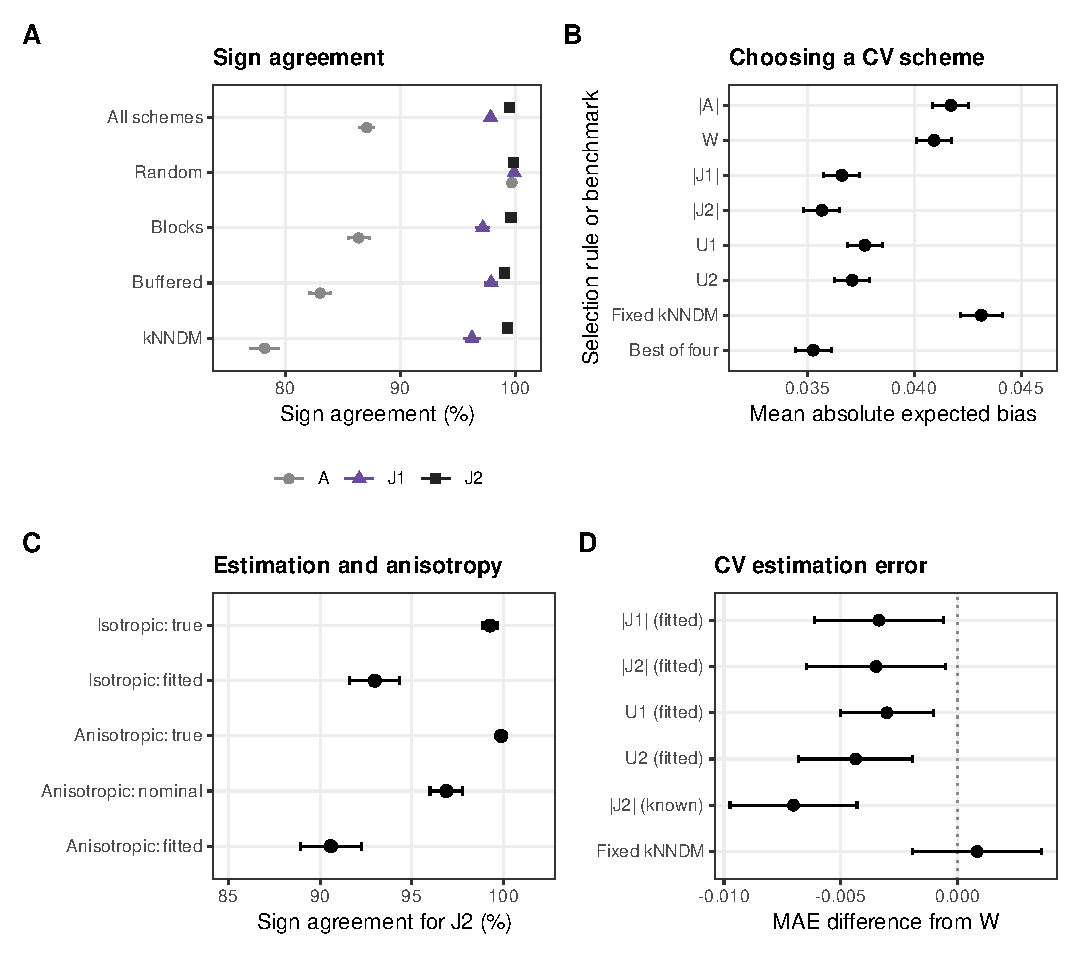
\includegraphics[width=\textwidth]{Fig2.pdf}
\caption{Diagnostics under known and estimated covariance. Bars show $\pm1.96$ MCSE. (A) Sign agreement for $|O|>0.01$ under known covariance. (B) Mean absolute expected bias after selection. Smaller values mean that expected CV MSE is closer to the prediction MSE at the target locations. Best of four averages the smallest true $|O|$ among the four candidates in each configuration; fixed kNNDM uses kNNDM throughout. Fixed random CV gives \BiasRandom, outside the plotted scale. (C) Sign agreement using the true covariance, specified parameters with direction ignored (nominal), or estimated isotropic covariance (fitted). (D) Paired MAE differences relative to selection by $W$; negative values favour the listed rule. Prediction uses estimated covariance throughout D; \emph{known} refers only to the correlation weights used for selection.}
\label{fig:reference}
\end{figure}

\subsection{Dependence on the prediction model}
\label{sec:sim-learners}
\paragraph{Design.}
The fourth experiment tests whether CV bias can change while $J_1$ and $J_2$ remain fixed. These contrasts are differences between validation and target averages of correlations and squared correlations, respectively, with the nearest training observation (Section~\ref{sec:correlation-model}). Let $X$ and $Z$ be independent Gaussian fields with unit variance and the same exponential correlation. We observe $X$ as a predictor and generate responses using unobserved $Z$ and independent observation noise $\epsilon$:
\begin{equation}
 Y=\sqrt{\alpha}X+\sqrt{0.9-\alpha}Z+\epsilon,\qquad
 \alpha\in\{0,0.3,0.6,0.9\},\quad\Var(\epsilon)=0.1.
\end{equation}
Increasing $\alpha$ makes $X$ explain more response variation while reducing the contribution of unobserved $Z$. Total spatial variance remains $0.9$, so the response correlation before accounting for $X$ stays unchanged. With locations and folds fixed, $J_1$ and $J_2$ calculated from this correlation also remain unchanged.

Across 480 independent field configurations, we compare prediction using the known mean $\sqrt{\alpha}X$, linear regression on $X$, random forests on $X$ \citep{wright2017ranger}, inverse-distance weighting using coordinates, and kriging with known mean and residual covariance. Within each configuration, the fields, training noise and folds are reused across $\alpha$.

For each simulated field, \emph{target loss} is the average squared error against the noise-free target responses plus the observation-noise variance, $0.1$. We subtract observed CV MSE from this loss and average the differences across fields. Positive values mean that CV underestimates target MSE on average. Online Resource 1 (Section~S5.1.2) gives design and scoring details.

\begin{samepage}
\paragraph{Results.}
For random CV with clustered sampling, scale $0.2$ and a target inside the sampled domain, mean $J_2$ stayed at \ConstantMarginal. For the random forest, we averaged target loss minus CV MSE over the 60 simulated fields in this setting. This average fell from \ForestZero\ at $\alpha=0$ to \ForestNine\ at $\alpha=0.9$ (MCSEs \ForestZeroSE\ and \ForestNineSE): random CV underestimated target MSE much less when $X$ was more informative. For inverse-distance weighting, which does not use $X$, the average difference changed little: \IDWZero\ to \IDWNine\ (Figure~\ref{fig:learners}).

\end{samepage}

The known-mean model predicts $\sqrt{\alpha}X$ directly, using the true coefficient supplied by the simulation. Its remaining error is $\sqrt{0.9-\alpha}Z+\epsilon$, which has mean zero and variance $1-\alpha$ at every location. Expected CV and target MSE are therefore both $1-\alpha$, so expected CV bias is zero. At $\alpha=0.9$, the $Z$ term disappears. The remaining noise is independent between locations, so neighbouring responses cannot predict it. Kriging therefore also predicts $\sqrt{0.9}X$.

These comparisons show why $J_2$ based on response correlation alone cannot determine CV bias: it does not account for how a prediction model uses $X$. All settings and schemes are shown in Online Resource 1 (Figure~S2).

\begin{figure}[!htbp]
\centering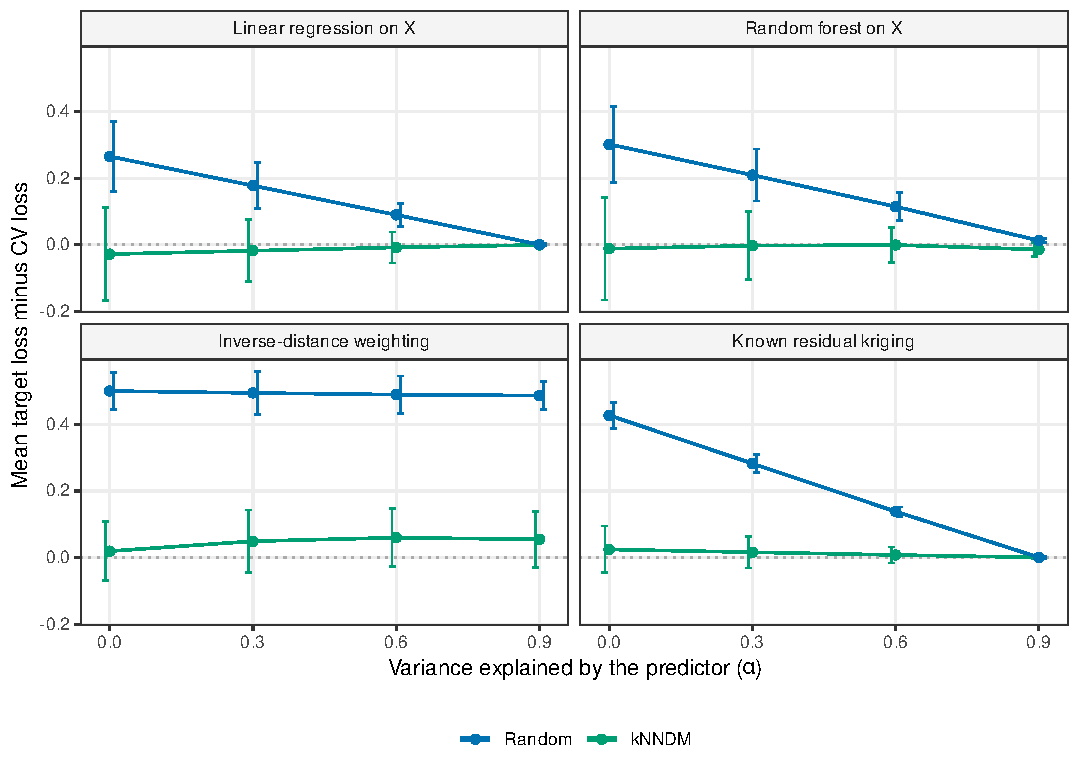
\includegraphics[width=\textwidth]{Fig3.pdf}
\caption{CV bias changes as the predictor $X$ becomes more informative, while response correlation stays fixed. This setting uses clustered sampling, scale $0.2$ and a target inside the sampled domain. Points average target loss minus CV MSE over 60 fields; positive values mean that CV underestimates target MSE. Bars show $\pm1.96$ MCSE. The contrast $J_2$, calculated from response correlation before accounting for $X$, stays constant for each scheme, with random-CV mean \ConstantMarginal. Inverse-distance weighting uses coordinates alone. Online Resource 1 (Figure~S2) includes all settings and the known-mean model, whose expected CV bias is zero.}
\label{fig:learners}
\end{figure}
\section{Application: cadmium concentrations in the Swiss Jura}
\label{sec:application}
\subsection{Data and prediction task}
The Jura soil survey measured trace-metal concentrations across a 14.5-km$^2$ area near La Chaux-de-Fonds, Switzerland \citep{atteia1994jura}. We use the 359-site dataset documented by \citet{goovaerts1997geostatistics} and distributed with \texttt{gstat} \citep{pebesma2004gstat}. The response is the natural logarithm of cadmium concentration, originally measured in mg/kg of topsoil. We retain the dataset's original split into 259 training sites and 100 reserved validation sites (Figure~\ref{fig:application}A). These reserved sites define our prediction target, with equal weights. Their measured concentrations allow a direct comparison between CV estimates and observed target MSE: the average squared prediction error at the 100 sites, on the log scale.

Ordinary kriging predicts log-cadmium using an estimated constant mean, exponential covariance and a nugget. Mean and covariance parameters are re-estimated using only the training observations available within each CV fold. A separate fit to all 259 training observations supplies the final prediction model. Target concentrations enter only the evaluation of its predictions.

\subsection{CV schemes and evaluation}
We compare the four five-fold schemes in Section~\ref{sec:cv-selection}: random folds, coordinate blocks, buffered blocks and kNNDM. The buffer is the median nearest-other-training distance. For this split, it removes no additional observations from the block training sets, so these two candidates coincide. We repeat fold construction 40 times with different random seeds. The training and target data and the final fitted model stay fixed. kNNDM returns the same folds every time.

We select the scheme with the smallest $W$ or $|J_2|$ and compare its CV score with observed target MSE at the 100 reserved sites. All candidates use the same full-training covariance estimate for $J_2$. The 40 repetitions describe variation due to fold allocation within this survey. Online Resource 1 (Section~S5.6.2) describes covariance estimation.

\subsection{Results and interpretation}
For the original 100 validation sites, random CV gives a closer estimate of observed target MSE than kNNDM. The observed target MSE is \JuraPublishedTarget: random CV averages \JuraPublishedRandomScore, whereas kNNDM gives \JuraPublishedKnnScore\ (Figure~\ref{fig:application}E). Random CV therefore underestimates the measured prediction error, while kNNDM overestimates it. Across the 40 repetitions, the mean absolute difference from observed target MSE is \JuraPublishedRandomMAE\ for random CV and \JuraPublishedKnnMAE\ for kNNDM. Both block schemes overestimate more strongly, averaging \JuraPublishedBlockScore.

Both diagnostic rules nevertheless select kNNDM in every repetition. Its validation distances most closely match the target distances (Figure~\ref{fig:application}B), and it has the smallest $W$ and $|J_2|$ (Figure~\ref{fig:application}C--D). Thus, the scheme that best matches these nearest-neighbour summaries does not give the most accurate CV estimate for this dataset.

The comparison changes when the target is the 100 northernmost sites. Both rules then select the block schemes, whose mean absolute difference from observed target MSE is \JuraNorthBlockMAE, compared with \JuraNorthRandomMAE\ for random CV. Adding a linear coordinate trend leaves these conclusions unchanged. Online Resource 1 (Section~S5.6.3, Table~S2 and Figure~S5) reports these checks and the random-holdout comparison.

\begin{figure}[p]
\centering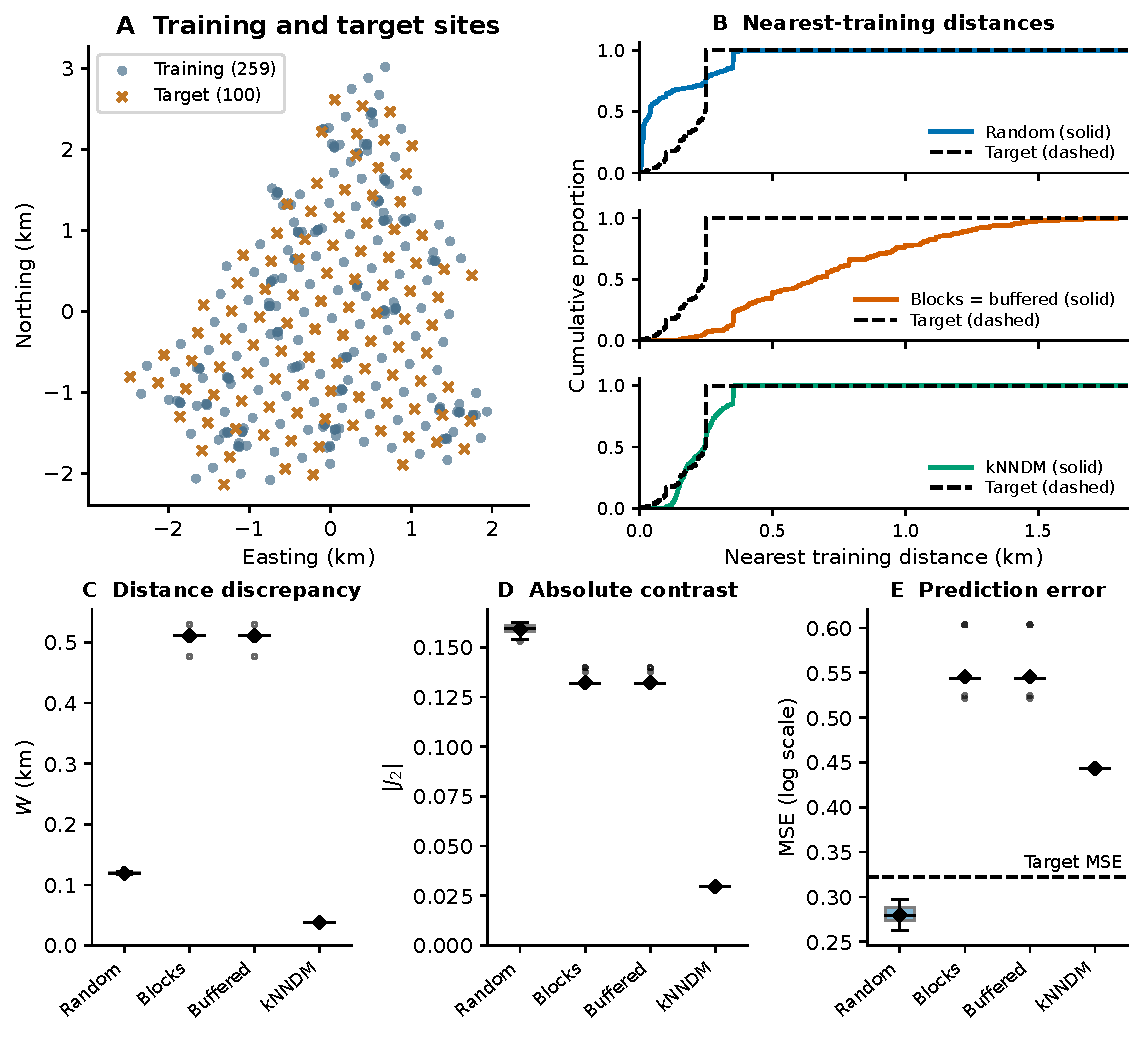
\includegraphics[width=\textwidth]{Fig4.pdf}
\caption{CV selection and observed prediction error for log-cadmium in the Swiss Jura. (A) The 259 training sites and 100 reserved target sites; coordinates are relative to the training-site centre. (B) In each comparison, the solid curve gives the proportion of validation sites with a nearest training neighbour within the indicated distance. The dashed curve gives the corresponding proportion for target sites. All three comparisons use the same axes and repetition 1; blocks and buffered blocks coincide. (C--D) $W$ and $|J_2|$: each rule selects the scheme with the smallest value. (E) CV MSE compared with observed target MSE (dashed line). In C--E, diamonds show means over 40 fold constructions, boxes show medians and interquartile ranges, and whiskers extend to observations within 1.5 interquartile ranges; points beyond them are shown separately. kNNDM gives identical values throughout. All MSEs use natural-log cadmium.}
\label{fig:application}
\end{figure}
\section{Discussion}
\label{sec:discussion}
Spatial CV is now standard for validating ecological and environmental maps, because random CV can severely understate prediction error when the target lies far from the data \citep{roberts2017cross,ploton2020spatial,meyer2022global}. Nearest-neighbour distance matching addresses this by making validation resemble prediction geographically \citep{mila2022nndm,linnenbrink2024knndm}. Our results clarify what such matching guarantees about prediction error and what it leaves undetermined. Three findings stand out. First, for Gaussian prediction from a single neighbour with known covariance, correlation-weighted matching is exactly the right criterion: $VJ_2$ equals the expected CV bias. Second, once prediction uses several observations, the information they supply jointly can bias CV even when nearest distances match perfectly. Third, correlation weighting improved scheme selection substantially when covariance was known, but by only \NestedReduction\% when covariance was estimated, and almost entirely in one setting.

\subsection{Guarantees and limits of nearest-neighbour matching}
The one-neighbour identity, $O_1=VJ_2$, explains why distances matter only through the correlation they imply. A shift in nearest distance changes prediction error when it changes the information a neighbour supplies. Where correlation decays rapidly, a small shift can remove most of that information. Where responses are weakly correlated at both validation and target distances, a large shift may have little effect. The Wasserstein distance $W$ weights every unit of distance equally and therefore cannot distinguish these situations, whereas $J_2$ weights CDF differences by the rate at which squared correlation declines (equation~\eqref{eq:weighting}). NNDM already incorporates dependence through an autocorrelation range \citep{mila2022nndm}; $J_2$ makes that dependence explicit and connects it directly to MSE.

The decomposition in equation~\eqref{eq:remainder} identifies what any nearest-neighbour summary leaves out. The remainder compares how much the other training observations reduce error during validation and at the target. It is small when the nearest observation largely screens the others from the prediction location, a property of kriging studied by \citet{stein2002screening}. Screening depends on the covariance model, the arrangement of observations and measurement error \citep{stein1999interpolation,stein2002screening}, so it cannot be assumed in general. The leave-one-out counterexample shows that the remainder alone can produce nonzero expected bias under a correctly specified model with perfectly matched nearest distances. Perfect distance matching is therefore not sufficient for unbiased validation. Nor can weights based only on nearest distances repair this: in the counterexample, such weights are all equal and leave the CV average unchanged.

The bound in equation~\eqref{eq:certificate} quantifies the gap. When its interval excludes zero, it determines the direction of expected CV bias under the stated covariance model. It contained every exact MSE difference in our simulations, but often included zero. This is the expected price of a guarantee that holds without further assumptions about how training observations are arranged.

\subsection{Evidence for correlation-weighted scheme selection}
The simulation evidence separates two targets of inference. With known covariance, selecting by $|J_2|$ rather than $W$ reduced mean absolute expected bias by \BiasReduction\%, and $J_2$ identified the direction of bias in \SignJTwo\% of evaluations with appreciable bias. This is the quantity that the theory addresses. With covariance estimated within each fold, the relevant quantity is the error of the observed CV score for the model fitted to that dataset, which also varies with the particular responses observed \citep{bates2024crossvalidation}. Here the reduction was \NestedReduction\%, concentrated in a setting with uniform sampling, a target extending beyond the sampled region, rapidly decaying correlation and low noise. Across the other 23 settings the average gain was negligible, and the ten-fold check gave an interval that included zero (Online Resource 1, Section~S5.4.1).

Two mechanisms explain this attenuation. First, estimated covariance degrades the contrast itself: sign agreement fell from \SensIsoTrue\% to \SensIsoEst\% under isotropic dependence, and fitted variograms sometimes placed the signal fraction or correlation scale at extreme values. Estimating covariance parameters also adds prediction error that plug-in calculations do not capture \citep{zimmerman1992mspe}. Second, observed CV scores vary between response datasets. The MAE of the scores selected by $W$ was \NestedMAEW, several times the mean absolute expected bias of \BiasW\ in the known-covariance study, although the two designs differ. When this variation is large relative to the differences in expected bias between candidate schemes, choosing the scheme with the best expected properties yields little gain for a single dataset. Comparisons between CV procedures are subject to substantial sampling variability more generally \citep{lei2020cvc,bates2024crossvalidation}.

The Jura application illustrates the practical consequence. Both diagnostics selected kNNDM for the original 100 validation sites, yet random CV was closer to the observed target MSE. With the northernmost sites as target, the selected block schemes were closer than random CV. The scheme that best matches nearest-neighbour summaries need not give the most accurate estimate for a particular survey, and the empirical comparison depends on the target. Because the application uses one survey, it cannot separate the additional-neighbour term from variation between response datasets.

\subsection{Spatial proximity is not data leakage}
The prediction model determines which spatial information matters. In Section~\ref{sec:sim-learners}, the bias of random CV for a random forest almost vanished as the predictor became informative, although response correlation and $J_2$ remained fixed. Response correlation describes dependence before accounting for predictors. Residual dependence, the model's use of predictors and whether target predictor values are represented in training all influence CV bias. Distance-based error profiles and area-of-applicability methods address the last two directly \citep{brenning2023profiles,meyer2021aoa}.

These diagnostics should therefore not be read as measures of data leakage. Leakage means using information that will not be available when the model is deployed \citep{kaufman2012leakage}. Nearby observations may be entirely legitimate at deployment; whether they are depends on the prediction task. The contrasts compare the spatial conditions of validation and prediction for a declared target. A contrast near zero does not certify that a CV estimate is accurate. It can arise from similar distance distributions, cancellation between positive and negative CDF differences, or weak correlation at all relevant distances. Like any single index, it could also become a target to optimise rather than evidence to interpret.

\subsection{Recommendations for practice}
The results support four recommendations for spatial validation.
\begin{enumerate}
\item \emph{Declare the prediction target.} CV bias is defined relative to target locations and their weights. Different targets in the same survey favoured different schemes in the Jura application.
\item \emph{Report the distance distributions together with correlation-weighted summaries.} The CDFs and $W$ describe the geographic mismatch. Comparing $|J_2|$ with $U_2$ reveals whether a small contrast arises from cancellation.
\item \emph{Treat diagnostics as conditional on a model.} $J_2$ and the bound rely on a Gaussian covariance model. Prediction error profiles, applicability assessments and residual analyses address what response correlation cannot \citep{brenning2023profiles,meyer2021aoa}.
\item \emph{Use probability sampling to estimate map accuracy.} For the error of a fixed map over a region, an independent probability sample supports design-based estimation without model assumptions \citep{wadoux2021spatial}.
\end{enumerate}

\subsection{Limitations and future directions}
The exact identities and bounds assume Gaussian responses with known mean and covariance. For non-Gaussian responses, such as presence--absence data, the relationship between correlation and MSE changes, and comparable results would require model-based extensions \citep{diggle1998model}. The simulations used exponential and Mat\'ern-$3/2$ covariance, a known mean and a fixed grid of designs, and overall MAE weights these settings equally. Inserting parameter estimates into the identities does not account for estimation uncertainty \citep{zimmerman1992mspe}, and inference after data-dependent scheme selection remains open.
The Jura analysis checked the covariance-fitting objective with a profile search over correlation scales, which left its findings unchanged (Online Resource 1, Section~S5.6.2). Rerunning all three estimated-covariance studies with the same search changed 5.5--9.4\% of variogram fits by more than 1\% in correlation scale, yet the selection results were essentially unaltered: the five-fold MAE reduction was 2.4\% (interval excluding zero), the ten-fold reduction 1.5\% (interval including zero), and the benefit remained concentrated in the same setting. Sign agreement with estimated covariance changed by 0.3 percentage points (Online Resource 1, Section~S5.4.2). The reported gains are therefore not an artefact of the fitting procedure, although they remain specific to the settings studied.

Several extensions follow directly from the decomposition. Covariance-based corrections modify the error estimator rather than choosing among schemes \citep{rabinowicz2022correlated}, and importance weighting adjusts for differences between sampled and target distributions \citep{sugiyama2007covariate,debruin2022clustered,brenning2026targetweighted}. Comparing these approaches with diagnostic scheme selection is an open problem. Any correction that improves on nearest-neighbour matching must represent the joint information supplied by several neighbours and the uncertainty in estimated dependence. Equation~\eqref{eq:remainder} specifies that term exactly.

Distance matching makes spatial validation resemble the intended prediction geographically. Our results show that this resemblance determines CV bias exactly only when prediction depends on a single neighbour and the covariance is known. Beyond that setting, credible accuracy assessment requires the prediction target, the prediction model and independent validation data, as well as the geometry of the sample.
\bmhead{Supplementary information}
Online Resource 1 contains the proofs, complete simulation designs, additional results, the profile-search refits and the reproduction records.

\section*{Statements and Declarations}
\begingroup\urlstyle{same}\emergencystretch=2em
\bmhead{Funding}
No funding was received for conducting this study.

\bmhead{Competing interests}
The author has no relevant financial or non-financial interests to disclose.

\bmhead{Ethics approval and consent to participate}
Not applicable. The study uses simulated data and a publicly available soil survey.

\bmhead{Consent for publication}
Not applicable.

\bmhead{Data availability}
The Jura soil data are distributed with the R package \texttt{gstat} and documented by \citet{goovaerts1997geostatistics}. The saved export, which retains all 359 site measurements and their original training--validation assignments, the simulation designs, random seeds and all saved results are available in the public reproduction repository, \url{https://github.com/olatunjijohnson/spCVAudit-paper}. Manuscript numbers and tables are generated from those results.

\bmhead{Code availability}
The reproduction repository, \url{https://github.com/olatunjijohnson/spCVAudit-paper}, provides the analysis code, figure scripts and archived source versions of the original implementation used for the computations (an R package developed under the working name \texttt{spLeakage}), together with the application code for the projection, log transformation, fold assignments, predictions and covariance-fitting checks. It retains the original computational implementation so that later package changes do not alter the reported results. The version accompanying this submission is tagged \texttt{ees-submission-v1}. The companion R package \texttt{spCVAudit}, available at \url{https://github.com/olatunjijohnson/spCVAudit} with documentation and tutorials at \url{https://olatunjijohnson.github.io/spCVAudit/}, implements the distance and correlation diagnostics, weighted targets, scheme comparisons and Gaussian reference calculations.

\bmhead{Author contributions}
Olatunji Johnson is the sole author and was responsible for conceptualisation, methodology, software, analysis, interpretation and writing.
\endgroup

\begin{thebibliography}{30}
\providecommand{\natexlab}[1]{#1}
\providecommand{\url}[1]{{#1}}
\providecommand{\urlprefix}{URL }
\providecommand{\doi}[1]{\url{https://doi.org/#1}}
\providecommand{\eprint}[2][]{\url{#2}}
 \bibcommenthead

\bibitem[{Arlot and Celisse(2010)}]{arlot2010survey}
Arlot S, Celisse A (2010) A survey of cross-validation procedures for model
  selection. Statistics Surveys 4:40--79. \doi{10.1214/09-SS054}

\bibitem[{Atteia et~al.(1994)Atteia, Dubois, and Webster}]{atteia1994jura}
Atteia O, Dubois JP, Webster R (1994) Geostatistical analysis of soil
  contamination in the {Swiss Jura}. Environmental Pollution 86(3):315--327.
  \doi{10.1016/0269-7491(94)90172-4}

\bibitem[{Bates et~al.(2024)Bates, Hastie, and
  Tibshirani}]{bates2024crossvalidation}
Bates S, Hastie T, Tibshirani R (2024) Cross-validation: What does it estimate
  and how well does it do it? Journal of the American Statistical Association
  119(546):1434--1445. \doi{10.1080/01621459.2023.2197686}

\bibitem[{Brenning(2023)}]{brenning2023profiles}
Brenning A (2023) Spatial machine-learning model diagnostics: a model-agnostic
  distance-based approach. International Journal of Geographical Information
  Science 37(3):584--606. \doi{10.1080/13658816.2022.2131789}

\bibitem[{Brenning and Suesse(2026)}]{brenning2026targetweighted}
Brenning A, Suesse T (2026) Aligning validation with deployment in spatial
  prediction: Target-weighted cross-validation.
  \doi{10.48550/arXiv.2603.29981},
  \urlprefix\url{https://arxiv.org/abs/2603.29981v3}, preprint,
  arXiv:2603.29981v3

\bibitem[{de~Bruin et~al.(2022)de~Bruin, Brus, Heuvelink, van
  Ebbenhorst~Tengbergen, and Wadoux}]{debruin2022clustered}
de~Bruin S, Brus DJ, Heuvelink GBM, et~al (2022) Dealing with clustered samples
  for assessing map accuracy by cross-validation. Ecological Informatics
  69:101665. \doi{10.1016/j.ecoinf.2022.101665}

\bibitem[{Diggle et~al.(1998)Diggle, Tawn, and Moyeed}]{diggle1998model}
Diggle PJ, Tawn JA, Moyeed RA (1998) Model-based geostatistics. Journal of the
  Royal Statistical Society: Series C (Applied Statistics) 47(3):299--350.
  \doi{10.1111/1467-9876.00113}

\bibitem[{Goovaerts(1997)}]{goovaerts1997geostatistics}
Goovaerts P (1997) Geostatistics for Natural Resources Evaluation. Oxford
  University Press, New York

\bibitem[{Hartigan and Wong(1979)}]{hartigan1979kmeans}
Hartigan JA, Wong MA (1979) Algorithm {AS} 136: A $k$-means clustering
  algorithm. Journal of the Royal Statistical Society Series C (Applied
  Statistics) 28(1):100--108. \doi{10.2307/2346830}

\bibitem[{Kaufman et~al.(2012)Kaufman, Rosset, Perlich, and
  Stitelman}]{kaufman2012leakage}
Kaufman S, Rosset S, Perlich C, et~al (2012) Leakage in data mining:
  Formulation, detection, and avoidance. ACM Transactions on Knowledge
  Discovery from Data 6(4):15:1--15:21. \doi{10.1145/2382577.2382579}

\bibitem[{Lei(2020)}]{lei2020cvc}
Lei J (2020) Cross-validation with confidence. Journal of the American
  Statistical Association 115(532):1978--1997.
  \doi{10.1080/01621459.2019.1672556}

\bibitem[{Linnenbrink et~al.(2024)Linnenbrink, Mil{\`a}, Ludwig, and
  Meyer}]{linnenbrink2024knndm}
Linnenbrink J, Mil{\`a} C, Ludwig M, et~al (2024) knndm cv: k-fold
  nearest-neighbour distance matching cross-validation for map accuracy
  estimation. Geoscientific Model Development 17(15):5897--5912.
  \doi{10.5194/gmd-17-5897-2024}

\bibitem[{Meyer and Pebesma(2021)}]{meyer2021aoa}
Meyer H, Pebesma E (2021) Predicting into unknown space? estimating the area of
  applicability of spatial prediction models. Methods in Ecology and Evolution
  12(9):1620--1633. \doi{10.1111/2041-210X.13650}

\bibitem[{Meyer and Pebesma(2022)}]{meyer2022global}
Meyer H, Pebesma E (2022) Machine learning-based global maps of ecological
  variables and the challenge of assessing them. Nature Communications 13:2208.
  \doi{10.1038/s41467-022-29838-9}

\bibitem[{Mil{\`a} et~al.(2022)Mil{\`a}, Mateu, Pebesma, and
  Meyer}]{mila2022nndm}
Mil{\`a} C, Mateu J, Pebesma E, et~al (2022) Nearest neighbour distance
  matching leave-one-out cross-validation for map validation. Methods in
  Ecology and Evolution 13(6):1304--1316. \doi{10.1111/2041-210X.13851}

\bibitem[{Panaretos and Zemel(2019)}]{panaretos2019wasserstein}
Panaretos VM, Zemel Y (2019) Statistical aspects of wasserstein distances.
  Annual Review of Statistics and Its Application 6:405--431.
  \doi{10.1146/annurev-statistics-030718-104938}

\bibitem[{Pebesma(2004)}]{pebesma2004gstat}
Pebesma EJ (2004) Multivariable geostatistics in {S}: the gstat package.
  Computers \& Geosciences 30(7):683--691. \doi{10.1016/j.cageo.2004.03.012}

\bibitem[{Ploton et~al.(2020)Ploton, Mortier, R{\'e}jou-M{\'e}chain, Barbier,
  Picard, Rossi, Dormann, Cornu, Viennois, Bayol, Lyapustin, Gourlet-Fleury,
  and P{\'e}lissier}]{ploton2020spatial}
Ploton P, Mortier F, R{\'e}jou-M{\'e}chain M, et~al (2020) Spatial validation
  reveals poor predictive performance of large-scale ecological mapping models.
  Nature Communications 11:4540. \doi{10.1038/s41467-020-18321-y}

\bibitem[{Rabinowicz and Rosset(2022)}]{rabinowicz2022correlated}
Rabinowicz A, Rosset S (2022) Cross-validation for correlated data. Journal of
  the American Statistical Association 117(538):718--731.
  \doi{10.1080/01621459.2020.1801451}

\bibitem[{Rasmussen and Williams(2006)}]{rasmussen2006gpml}
Rasmussen CE, Williams CKI (2006) Gaussian Processes for Machine Learning. MIT
  Press, \urlprefix\url{https://gaussianprocess.org/gpml/}

\bibitem[{Roberts et~al.(2017)Roberts, Bahn, Ciuti, Boyce, Elith,
  Guillera-Arroita, Hauenstein, Lahoz-Monfort, Schr{\"o}der, Thuiller, Warton,
  Wintle, Hartig, and Dormann}]{roberts2017cross}
Roberts DR, Bahn V, Ciuti S, et~al (2017) Cross-validation strategies for data
  with temporal, spatial, hierarchical, or phylogenetic structure. Ecography
  40(8):913--929. \doi{10.1111/ecog.02881}

\bibitem[{Stein(1999)}]{stein1999interpolation}
Stein ML (1999) Interpolation of Spatial Data: Some Theory for Kriging.
  Springer, New York, \doi{10.1007/978-1-4612-1494-6}

\bibitem[{Stein(2002)}]{stein2002screening}
Stein ML (2002) The screening effect in kriging. The Annals of Statistics
  30(1):298--323. \doi{10.1214/aos/1015362194}

\bibitem[{Sugiyama et~al.(2007)Sugiyama, Krauledat, and
  M{\"u}ller}]{sugiyama2007covariate}
Sugiyama M, Krauledat M, M{\"u}ller KR (2007) Covariate shift adaptation by
  importance weighted cross validation. Journal of Machine Learning Research
  8:985--1005. \urlprefix\url{https://jmlr.org/papers/v8/sugiyama07a.html}

\bibitem[{Wadoux et~al.(2021)Wadoux, Heuvelink, de~Bruin, and
  Brus}]{wadoux2021spatial}
Wadoux AMJC, Heuvelink GBM, de~Bruin S, et~al (2021) Spatial cross-validation
  is not the right way to evaluate map accuracy. Ecological Modelling
  457:109692. \doi{10.1016/j.ecolmodel.2021.109692}

\bibitem[{Wang et~al.(2023)Wang, Hopkins, Hallman, Robinson, and
  Hutchinson}]{wang2023geospatial}
Wang J, Hopkins LM, Hallman TA, et~al (2023) Cross-validation for geospatial
  data: Estimating generalization performance in geostatistical problems.
  Transactions on Machine Learning Research
  \urlprefix\url{https://openreview.net/forum?id=VgJhYu7FmQ}

\bibitem[{Wang et~al.(2025)Wang, Khodadadzadeh, and
  Zurita-Milla}]{wang2025dissimilarity}
Wang Y, Khodadadzadeh M, Zurita-Milla R (2025) A dissimilarity-adaptive
  cross-validation method for evaluating geospatial machine learning
  predictions with clustered samples. Ecological Informatics 90:103287.
  \doi{10.1016/j.ecoinf.2025.103287}

\bibitem[{Wright and Ziegler(2017)}]{wright2017ranger}
Wright MN, Ziegler A (2017) ranger: A fast implementation of random forests for
  high dimensional data in {C++} and {R}. Journal of Statistical Software
  77(1):1--17. \doi{10.18637/jss.v077.i01}

\bibitem[{Yuval and Rosset(2025)}]{yuval2025classification}
Yuval O, Rosset S (2025) Cross validation for correlated data in classification
  models. In: Proceedings of the 28th International Conference on Artificial
  Intelligence and Statistics, pp 1702--1710,
  \urlprefix\url{https://proceedings.mlr.press/v258/yuval25a.html}

\bibitem[{Zimmerman and Cressie(1992)}]{zimmerman1992mspe}
Zimmerman DL, Cressie N (1992) Mean squared prediction error in the spatial
  linear model with estimated covariance parameters. Annals of the Institute of
  Statistical Mathematics 44(1):27--43. \doi{10.1007/BF00048668}

\end{thebibliography}
\end{document}
